\documentclass{beamer}

\usepackage[utf8]{inputenc}
\usepackage[T1]{fontenc}

\usepackage[english]{babel}
\usepackage{amsmath}
\usepackage{cleveref}
\usepackage{amssymb}
\usepackage{mathtools}

%%Numbers, expectation
\newcommand{\N}{\mathbb{N}}
\newcommand{\E}{\mathbb{E}}
\renewcommand{\P}{\mathbb{P}}
\newcommand{\Var}{\mathbb{V}}
\newcommand{\R}{\mathbb{R}}
\newcommand{\D}{\mathcal{D}}
\newcommand{\B}{\mathcal{B}}
\newcommand{\Dh}{\D_h}
\renewcommand{\phi}{\varphi}
\newcommand*\diff{\mathop{}\!\mathrm{d}} % integral

%% mathoperator
\DeclareMathOperator*{\argmax}{arg\,max}
\DeclareMathOperator*{\argmin}{arg\,min}
\DeclareMathOperator*{\dom}{dom}
\DeclareMathOperator*{\sign}{sign}
\DeclareMathOperator*{\diag}{diag}

\DeclareMathOperator*{\Cov}{Cov}
\DeclareMathOperator*{\Cor}{Corr}
\DeclareMathOperator*{\Id}{Id}

%proximal operator
\newcommand{\prox}[3][]{\operatorname{prox}^{#1}_{#2}\left(#3 \right)}

\usepackage{xcolor}

%% sort citations by increasing number
\usepackage[sort,nocompress]{cite}

\usepackage{graphicx}% http://ctan.org/pkg/graphicx
\graphicspath{{../figures/}{../../figures}{../../memes}} %Setting the graphicspath
\usepackage{caption,subcaption}

\usepackage{tikz}
\usepackage{pgfplots}
\usetikzlibrary{backgrounds}
\usetikzlibrary{intersections}
\usepgfplotslibrary{fillbetween}

% \usepackage[right]{showlabels}


%%
\theoremstyle{plain}
\newtheorem{prop}{Proposition}[section]
\newtheorem{algo}{Algorithm}[section]
\newtheorem{assumption}{Assumption}
\theoremstyle{remark}
\newtheorem{remark}{Remark}[section]

% cref
\crefname{assumption}{Assumption}{Assumptions}
\crefname{equation}{}{}

\usepackage{autonum}

\usepackage{bm} %% bold math symbols

\usepackage{bbm} %% for \mathbbm{1}


% algorithmic environment
\usepackage{algorithm}
\usepackage[noend]{algpseudocode}

% for some reason this was required on one void linux installation (but not the other)
\usepackage{sansmathaccent}
\pdfmapfile{+sansmathaccent.map}

\author{Axel Böhm}

% shows which section we're in
\usetheme{Darmstadt}

% page number
\setbeamertemplate{footline}[frame number]
\setbeamercolor{page number in head/foot}{fg=gray}


% display things like onslide or visible already before but grayed out
\setbeamercovered{transparent}

% set the itemize item symbol as a diamond
\setbeamertemplate{itemize item}{$\diamond$}
% set the itemize subitem symbol as a triangle
\setbeamertemplate{itemize subitem}{$\blacktriangleright$}

% set the enumerate item symbol as a roman numbers
\setbeamertemplate{enumerate item}{(\roman{enumi})}


\author{Axel Böhm}

% shows which section we're in
\usetheme{Darmstadt}

% page number
\setbeamertemplate{footline}[frame number]
\setbeamercolor{page number in head/foot}{fg=gray}


% display things like onslide or visible already before but grayed out
\setbeamercovered{transparent}

% set the itemize item symbol as a diamond
\setbeamertemplate{itemize item}{$\diamond$}
% set the itemize subitem symbol as a triangle
\setbeamertemplate{itemize subitem}{$\blacktriangleright$}

% set the enumerate item symbol as a roman numbers
\setbeamertemplate{enumerate item}{(\roman{enumi})}

\usepackage{changepage}
% https://openai.com/blog/deep-double-descent/

\title{(Sub)-gradient method}
\date{\today}

\begin{document}
\maketitle
\frame{\tableofcontents}

\section{Intro}%

\begin{frame}
  \frametitle{Spoiler: Smooth vs.\ nonsmooth}
  We consider the convex optimization problem
  \begin{equation}
    \min_x \, f(x)
  \end{equation}
  \vspace{-0.5cm}
  \begin{block}{}
    \begin{equation}
      x_{k+1} = x_k - \alpha g_k
    \end{equation}
  \end{block}
  \begin{adjustwidth}{-1.5em}{-1.5em}
    \begin{minipage}{0.52\textwidth}
      \begin{block}{}
        \begin{itemize}
          \item If $f$ is \textcolor{blue}{smooth} we take $g_k = \nabla f(x_k)$ $\rightarrow$ \textbf{Gradient Descent}.
          \item stepsize can be constant $1/L$ (smoothness constant)
          \item convergence rate $f(x_k)-f^* = \mathcal{O}(1/k)$
        \end{itemize}
      \end{block}
    \end{minipage}
    \hfill
    \begin{minipage}{0.52\textwidth}
      \begin{block}{}
        \begin{itemize}
          \item If \textcolor{blue}{not} we take $g_k$ a \textit{subgradient} $\rightarrow$ \textbf{Subgradient method}.
          \item stepsize has to be chosen \emph{small or decreasing} $\approx 1/\sqrt{k}$
          \item convergence rate is \emph{worse} $f(x_k)-f^* = \mathcal{O}(1/\sqrt{k})$
        \end{itemize}
      \end{block}
    \end{minipage}
  \end{adjustwidth}
\end{frame}

\begin{frame}
  \frametitle{Intuition behind GD}
  \begin{itemize}
    \item derivative (gradient) points in the direction of steepest ascent
          $\rightarrow$ GD is also called \textbf{steepest descent}
    \item GD update is equivalent to
          \begin{equation}
            x_{k+1} = \argmin_{x\in \R^d} \Big\{ \underbrace{f(x_k) + \langle \nabla f(x_k), x-x_k \rangle }_{\text{linearization of $f$}}+ \frac{1}{2 \alpha} \Vert x-x_k \Vert^2 \Big\}
          \end{equation}
          \begin{itemize}
            \item solves a linear model of $f$
            \item minimizing unconstrained linear models is no good
            \item so we add a ``proximity term''
          \end{itemize}
  \end{itemize}
\end{frame}


\section{Subgradient theory}%

\begin{frame}
  \frametitle{Subgradients}
  What if $f$ is not differentiable?
  \begin{definition}
    $g \in \R^d$ is a \textcolor{blue}{subgradient} of $f$ at $x$ if
    \begin{equation}
      f(y) \ge f(x) + g^T (y-x)
    \end{equation}
  \end{definition}
  \begin{figure}[ht]
    \centering
    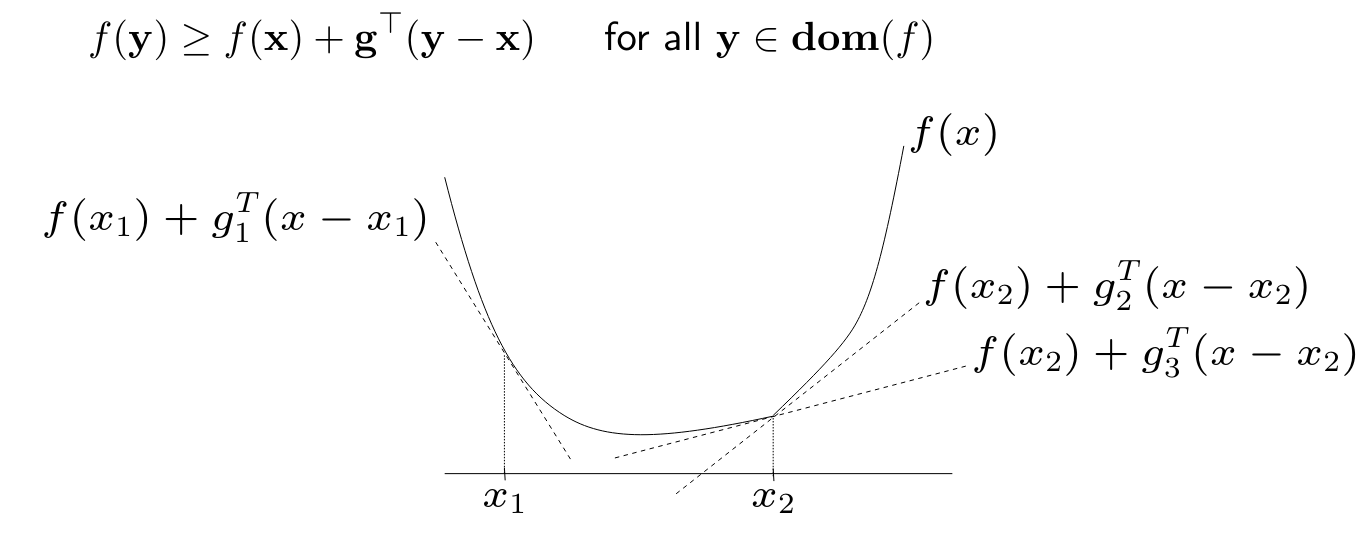
\includegraphics[width=\textwidth,height=\textheight,keepaspectratio]{subgradients}
    % \caption{\label{fig:label} }
  \end{figure}
\end{frame}

\begin{frame}
  \frametitle{Subgradients II}
  \begin{definition}
    The \textcolor{blue}{subdifferential} $\partial f(x)$ is the \emph{set of all subgradients} of $f$ at $x$.
  \end{definition}
  Example
  \begin{figure}[ht]
    \centering
    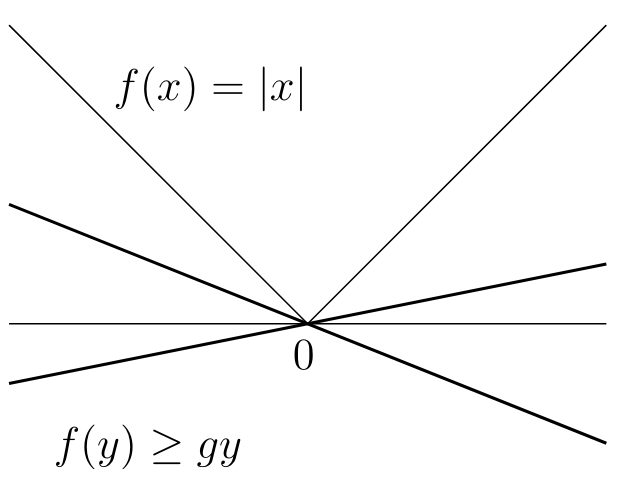
\includegraphics[width=0.5\textwidth,keepaspectratio]{subdifferential}
    % \caption{\label{fig:label} }
  \end{figure}
  Subgradient condition at $x=0$ is $f(y)\ge f(0) + g(y-0) = gy$.
  \textcolor{purple}{What is $\partial f(0)$?}
\end{frame}

\begin{frame}
  \frametitle{Subgradients III}
  \begin{lemma}%
    If $f$ is differentiable at $x$ then $\partial f(x) \subset \{\nabla f(x)\}$
  \end{lemma}
  So either one subgradient or none.\\
  \begin{minipage}{0.48\textwidth}
    \begin{figure}[ht]
      \centering
      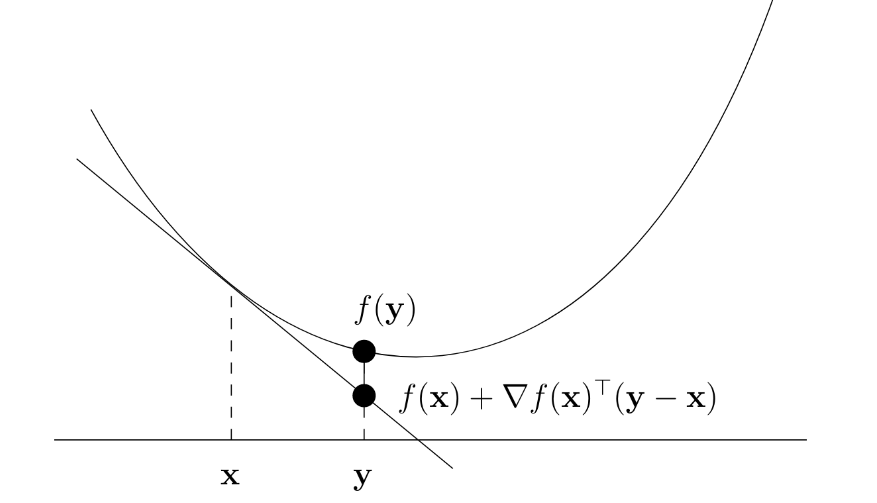
\includegraphics[width=\textwidth,keepaspectratio]{graph_above_tangent}
      % \caption{\label{fig:label} }
    \end{figure}
  \end{minipage}
  \hfill
  \begin{minipage}{0.48\textwidth}
    \begin{figure}[ht]
      \centering
      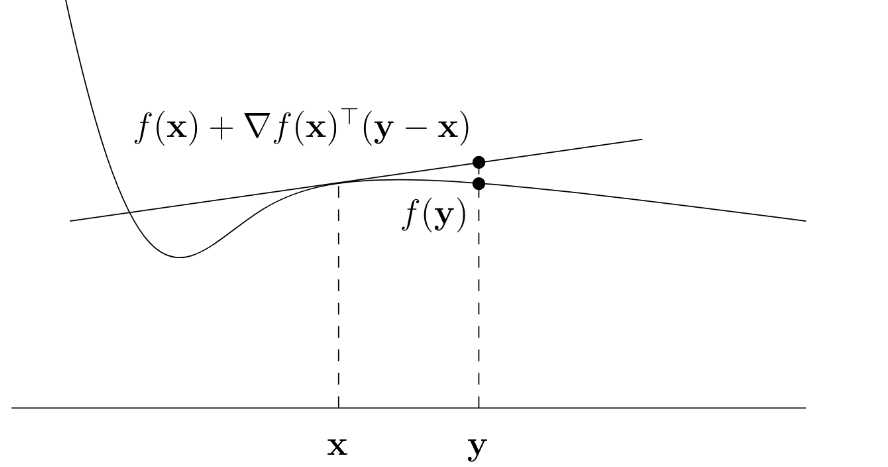
\includegraphics[width=\textwidth,keepaspectratio]{differentiable_function}
      % \caption{\label{fig:label} }
    \end{figure}
  \end{minipage}
\end{frame}

\begin{frame}
  \frametitle{Subgradient characterization of convexity}
  \begin{lemma}%
    A function $f: \R^d \to \R$ is convex \textit{if and only if} $\partial f(x)$ is not empty for all $x$.
  \end{lemma}
  \begin{figure}[ht]
    \centering
    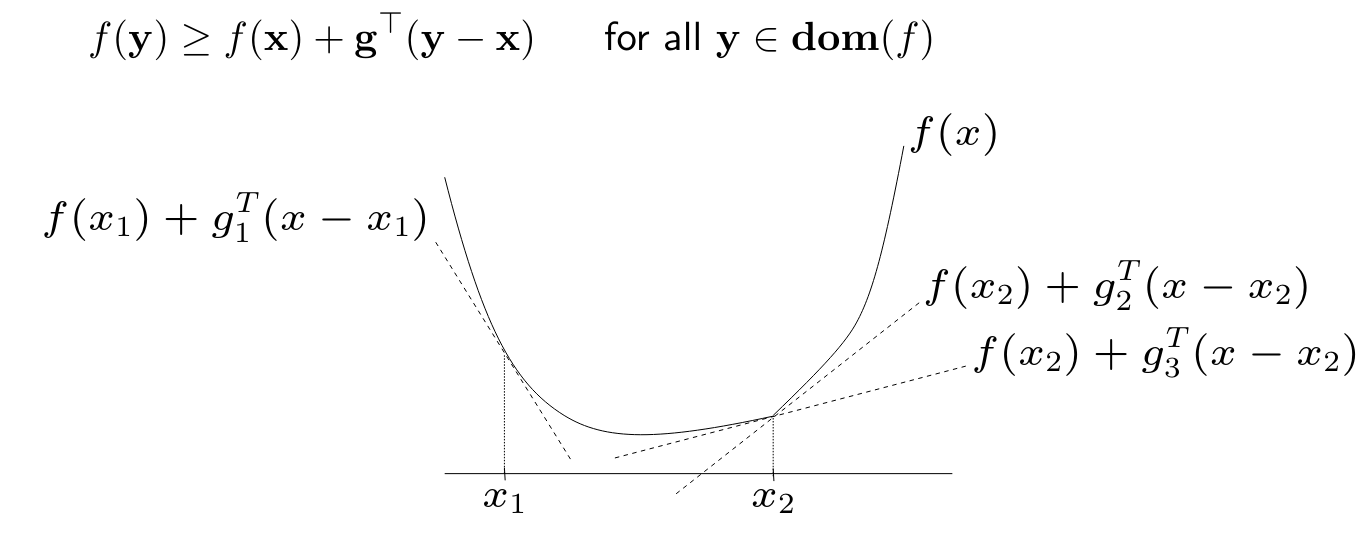
\includegraphics[width=\textwidth,keepaspectratio]{subgradients}
    \caption{Subgradients at every point.}
  \end{figure}
\end{frame}

\begin{frame}
  \frametitle{Lipschitz = bounded subgradients}
  \begin{definition}
    We call $f$ $L$-Lipschitz (continuous) if
    \begin{equation}
      \Vert f(x)-f(y) \Vert \le L \Vert x-y \Vert.
    \end{equation}
  \end{definition}
  \begin{lemma}%
    Let $f$ be convex. Then the following two are equivalent.
    \begin{enumerate}
      \item All \textbf{subgradients are uniformly bounded}.
            \begin{equation}
              \Vert g \Vert \le L \quad \forall x, \forall g \in \partial f(x)
            \end{equation}
      \item $f$ is $L$-Lipschitz
    \end{enumerate}
  \end{lemma}
\end{frame}

\begin{frame}
  \frametitle{Subgradient optimality condition}
  \begin{lemma}%
    Let \textcolor{blue}{$0 \in \partial f(\bar{x})$}, then $\bar{x}$ is a \textcolor{blue}{global minimum}.
  \end{lemma}
  \begin{proof}
    By the definition of subgradients, $g=0 \in \partial f(\bar{x})$ gives
    \begin{equation}
      f(y) \ge f(\bar{x}) + g^T(y-\bar{x}) = f(\bar{x}).
    \end{equation}
  \end{proof}
\end{frame}


\section{Convergence subgradient method}%
\label{sec:}

\begin{frame}
  \frametitle{Convergence statement: Subgradient method}
  \textcolor{gray}{We assume there exists minimizer $x^*$ and we write $f^*=f(x^*)$.}
  \begin{theorem}
    $f$ is convex, subgradients are bounded $\Vert g(x) \Vert \le G$ for all $g(x)\in \partial f(x)$. Then,
    \begin{equation}
<<<<<<< HEAD
      f(\bar{x}_k) - f^* \le \frac{\Vert x_1-x^*\Vert G}{\sqrt{k}}
=======
      f(\bar{x}_k) - f^* \le \frac{\Vert x_0-x^*\Vert^2 G}{\sqrt{k}}
>>>>>>> refs/remotes/origin/main
    \end{equation}
    for the \textbf{averaged} iterates $\bar{x}_k = \frac{1}{k} \sum_{i=0}^{k-1} x_i $
  \end{theorem}
  \begin{itemize}
    \item Also holds for the \textbf{``best''} iterate.
    \item \textcolor{blue}{Dimension independent!} (no $d$)
  \end{itemize}
\end{frame}

\begin{frame}
  \frametitle{Proof}
  \vspace{-0.5cm}
  \begin{equation}
    \begin{aligned}
      \Vert x_{k+1} - x^* \Vert^2 &\le \Vert x_k - \alpha g_k - x^* \Vert^2 \\
      &= \Vert x_k-x^* \Vert^2 + 2 \alpha \langle g_k, x^*-x_k \rangle + \alpha^2 \Vert g_k \Vert^2.
    \end{aligned}
  \end{equation}
  Using the \textbf{subgradient inequality} $\langle g_k , x^* -x_k \rangle \le f(x^*) - f(x_k)$
  % \begin{equation}
  %   \langle g_k , x^* -x_k \rangle \le f(x^*) - f(x_k)
  % \end{equation}
  \begin{equation}
    \Vert x_{k+1} - x^* \Vert^2 \le \Vert x_k-x^* \Vert^2 + 2 \alpha(f(x^*) - f(x_k)) + \alpha^2 \Vert g_k \Vert^2.
  \end{equation}
  Summing up (telescoping) yields
  \begin{equation}
    \label{eq:telescoping}
    2\sum_{i=0}^{k-1}  \alpha(f(x_i) - f(x^*)) + \Vert x_{k} - x^* \Vert^2 \le \Vert x_0-x^* \Vert^2 +  \alpha^2 \sum_{i=0}^{k-1} \Vert g_k \Vert^2.
  \end{equation}
  Via the \emph{bounded subgradient} assumption
  \begin{equation}
    2\sum_{i=0}^{k-1}  \alpha(f(x_i) - f(x^*)) \le \Vert x_0-x^* \Vert^2 +  \alpha^2 k G^2.
  \end{equation}
\end{frame}

\begin{frame}
  \frametitle{Proof [contd]}
  We divide by $2\alpha$ and $k$
  \begin{equation}
    \frac{1}{k}\sum_{i=0}^{k-1}  f(x_i) - f^*  \le \frac{1}{2 \alpha k} \Vert x_0-x^* \Vert^2 +  \frac{\alpha G^2}{2}
  \end{equation}
  Using Jensens inequality (convexity with more than $2$ points)
  \begin{equation}
    \sum_{i=0}^{k-1} \frac{1}{k} f(x_i) \ge \sum_{i} f \left( \frac{1}{k}\sum_{i=0}^{k-1}x_i \right)
  \end{equation}
  we obtain
  \begin{equation}
    f(\bar{x}_k) - f^*  \le \frac{1}{2 \alpha k} \Vert x_0-x^* \Vert^2 + \frac{\alpha G^2}{2}.
  \end{equation}

\end{frame}

\begin{frame}
  \frametitle{How to choose the stepsize?}
  We have
 \begin{equation}
    f(\bar{x}_k) - f^*  \le \frac{1}{2 \alpha k} \Vert x_0-x^* \Vert^2 + \alpha G^2.
  \end{equation}
  Choose $\alpha$ such that \textit{RHS is minimized}, i.e.\
  \begin{equation}
    \alpha = \frac{\Vert x_0-x^*\Vert }{G \sqrt{k}},
  \end{equation}
  which gives
  % Clearly $\alpha_i = \ell_2 \textbackslash \ell_1$ leads convergence, for example $1/i$.
  % However, $\alpha = \mathcal{O}(1/\sqrt{i})$ gives
  % \begin{equation}
  %   \sum \alpha_i = (\frac{1}{\sqrt{1}} + \frac{1}{\sqrt{2}} + \cdots +  \frac{1}{\sqrt{k}}) > \sqrt{k}
  %   \sum \alpha^2 = (\frac{1}{1} + \frac{1}{2} + \cdots + \frac{1}{k}) \approx \log(k)
  % \end{equation}

  \begin{equation}
    f(\bar{x}_k) - f^* \le \frac{\Vert x_0-x^*\Vert G }{\sqrt{k}}. \qed
  \end{equation}
  When ignoring constants (and focusing on the rate) we sometimes write
  \begin{equation}
    \mathcal{O}\left(\frac{1}{\sqrt{k}}\right).
  \end{equation}
\end{frame}

\begin{frame}
  \frametitle{Complexity}
  For convex Lipschitz functions we require \textcolor{blue}{$\mathcal{O}(\epsilon^{-2})$} iterations. For $D:= \Vert x_0 -x^* \Vert$
  \begin{equation}
    f(\bar{x}_k) - f^* \le \frac{D G}{\sqrt{k}}
  \end{equation}
  \textbf{Q:} How many iterations to get
  \begin{equation}
    f(\bar{x}_k) - f^* \le \epsilon ?
  \end{equation}
  \textbf{A:} We get this if
  \begin{equation}
    \frac{D G}{\sqrt{k}} \le \epsilon
  \end{equation}
  Equivalently
  \begin{equation}
    k \ge \frac{D^2 G^2}{\epsilon^2}.
  \end{equation}
\end{frame}



\begin{frame}
  \frametitle{Polyak stepsize}
  Let's revisit the convergence proof of the subgradient method
  \begin{equation}
    \begin{aligned}
      \Vert x_{k+1} - x^* \Vert^2 &\le \Vert x_k - \alpha_k g_k - x^* \Vert^2 \\
      &= \Vert x_k-x^* \Vert^2 + 2 \alpha \langle g_k, x^*-x_k \rangle + \alpha^2 \Vert g_k \Vert^2\\
      &\le \Vert x_k-x^* \Vert^2 + 2 \alpha (f^* - f(x_k))+ \alpha^2 \Vert g_k \Vert^2.
    \end{aligned}
  \end{equation}
  Can we pick $\alpha$ such that the RHS is minimized?
  \begin{equation}
    \min_\alpha \, \alpha^2 \Vert g_k \Vert^2 + 2 \alpha (f^* - f(x_k))
  \end{equation}
  gives
  \begin{equation}
    \alpha_k^* = \frac{f(x_k)-f^*}{\Vert g_k \Vert^2}
  \end{equation}
  \begin{equation}
      \Vert x_{k+1} - x^* \Vert^2 = \Vert x_k-x^* \Vert^2 - {\left( \frac{f(x_k)-f^*}{\Vert g_k \Vert} \right)}^2
  \end{equation}
\end{frame}

\begin{frame}
  \frametitle{Polyak stepsize [contd]}
  \begin{itemize}
    \item Requires us to know the optimal objective function value
    \item can be the case in certain setting:
          separable data, feasibility problems
    \item modern deep learning interpolation setting
  \end{itemize}
  \begin{figure}[ht]
    \centering
    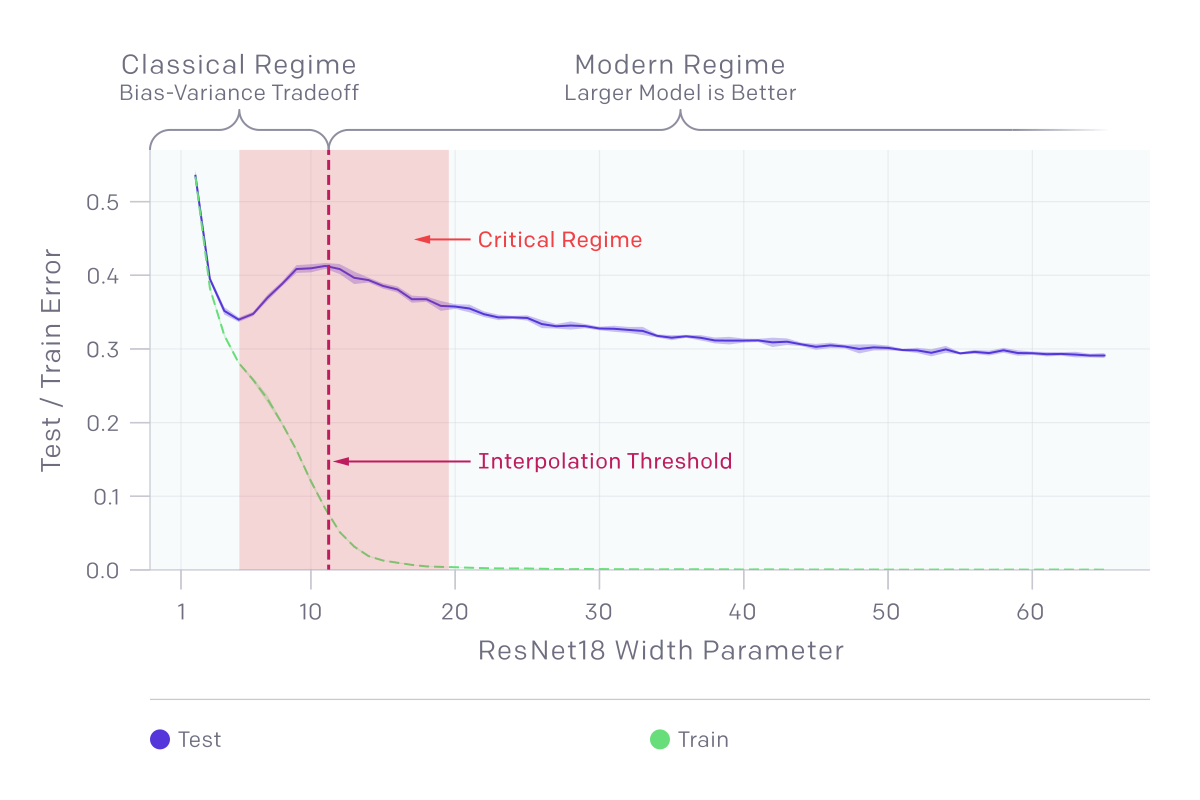
\includegraphics[width=0.7\textwidth]{modern-regime}
    \caption{from openai.com}
  \end{figure}
\end{frame}


\section{Smooth case}%
\label{sec:}

\begin{frame}
  \frametitle{Can we do better if the function is smooth?}
  \begin{definition}
    We call a function $L$-\textcolor{blue}{smooth} if
    \begin{equation}
      f(y) \le f(x) + \langle \nabla f(x), y-x \rangle + \frac{L}{2} \Vert y-x \Vert^2.
    \end{equation}
  \end{definition}
  \begin{center}
    \textit{Can be upper bounded by a quadratic.}
  \end{center}
  \begin{lemma}%
    If the gradient of $f$ is $L$-Lipschitz
    \begin{equation}
      \Vert \nabla f(x)- \nabla f(y) \Vert \le L \Vert x-y \Vert.
    \end{equation}
    then it is also $L$-smooth.
  \end{lemma}
  Note: Definition does not require convexity.
\end{frame}


\begin{frame}
  \frametitle{Smoothness}
  If $f$ is convex we get upper and lower bound:

  \begin{figure}[ht]
    \centering
    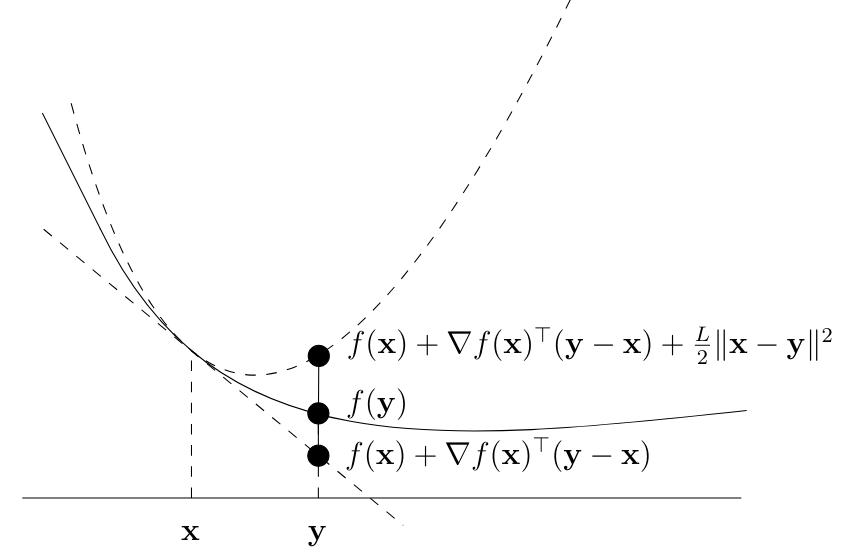
\includegraphics[width=\textwidth,keepaspectratio]{smoothness}
    % \caption{\label{fig:label} }
  \end{figure}
\end{frame}


\begin{frame}
  \frametitle{Smooth vs. Lipschitz}
  \begin{itemize}
    \item Bounded (sub)gradients $\Leftrightarrow$ Lipschitz continuity of $f$
    \item Smoothness $\Leftrightarrow$ Lipschitz continuity of $\nabla f$ (if convex)
  \end{itemize}

  \begin{lemma}%
    Let $f$ be convex and differentiable, then the following are \textit{equivalent}
    \begin{enumerate}
      \item $f$ is smooth with parameter $L$
      \item $\nabla f$ is $L$-Lipschitz
    \end{enumerate}
  \end{lemma}
\end{frame}


\begin{frame}
  \frametitle{Sufficient decrease}
  \begin{lemma}%
    If $f$ is $L$-smooth with stepsize $\alpha = 1/L$, then gradient descent satisfies
    \begin{equation}
      f(x_{k+1}) \le f(x_k) - \frac{1}{2L} \Vert \nabla f(x_k) \Vert^2
    \end{equation}
  \end{lemma}
  \begin{proof}
    \begin{equation}
      \begin{aligned}
        f(x_{k+1}) &\le f(x_k) + \langle \nabla f(x_k), x_{k+1}-x_k \rangle + \frac{L}{2}\Vert x_{k+1}-x_k \Vert^2 \\
        &= f(x_k) - \alpha \Vert \nabla f(x_k) \Vert^2 + \frac{\alpha^2 L}{2} \Vert \nabla f(x_k) \Vert^2 \\
        &= f(x_k) - \left(\frac{1}{L} - \frac{1}{2L}\right) \Vert \nabla f(x_k) \Vert^2
      \end{aligned}
    \end{equation}
  \end{proof}
\end{frame}


\begin{frame}
  \frametitle{Smooth convex functions}
  \begin{theorem}
    Let $f: \R^d \to \R$ be convex and $L$-smooth and the stepsize $\alpha=1/L$, then
    \emph{gradient descent} yields
    \begin{equation}
      f(x_k)-f^* \le \frac{L}{2k}\Vert x_0-x^* \Vert^2.
    \end{equation}
  \end{theorem}
  \begin{itemize}
    \item holds for last iterate
    \item independet of dimension $d$
  \end{itemize}
\end{frame}

\begin{frame}
  \frametitle{Complexity of gradient method}
  Denote $D^2 := \Vert x_1- x^* \Vert^2$
  \begin{equation}
    \text{iteration: } k \ge \frac{D^2 L}{2 \epsilon} \Rightarrow \text{error} \le \frac{L D^2}{2 k} \le \epsilon
  \end{equation}
  Given error $\epsilon=0.01$ results in
  \begin{itemize}
    \item $50 \cdot D^2 L$ iterations for \textit{smooth} case
      \item $10 000 \cdot D^2 G^2$ for nonsmooth but Lipschitz
  \end{itemize}

  What if we don't know $L$?
\end{frame}

\begin{frame}
  \frametitle{Proof of $\mathcal{O}(\epsilon^{-1})$ for smooth functions}
    Subgradient analysis gave us
    \begin{equation}
      \sum_{i=0}^{k-1} (f(x_i) - f^*) \le \frac{1}{2 \alpha}\Vert x_0-x^* \Vert^2 +  \frac{\alpha}{2} \sum_{i=0}^{k-1}  \Vert g_k \Vert^2,
    \end{equation}
    see~\eqref{eq:telescoping}. This time we use \textcolor{blue}{sufficient decrease} to bound gradient norm
    \begin{equation}
      \frac{1}{2 L} \sum_{i=0}^{k-1} \Vert \nabla f(x_k) \Vert^2 \le \sum_{i=0}^{k-1} (f(x_i) - f(x_{i+1})) = f(x_0) - f(x_k)
    \end{equation}
    Combining the above two (with $\alpha=1/L$)
    \begin{equation}
      \begin{aligned}
        \sum_{i=0}^{k-1} (f(x_i) - f^*)  &\le \frac{L}{2} \Vert x_0-x^* \Vert^2 +  \frac{1}{2L} \sum_{i=0}^{k-1}  \Vert g_k \Vert^2 \\
        &\le \frac{L}{2} \Vert x_0-x^* \Vert^2 + f(x_0) - f(x_k)
      \end{aligned}
    \end{equation}
\end{frame}

\begin{frame}
  \frametitle{Proof II}
  By rewriting:
    \begin{equation}
      \sum_{\textcolor{red}{i=1}}^{\textcolor{red}{k}} (f(x_i) - f^*) \le \frac{L}{2} \Vert x_0-x^* \Vert^2
    \end{equation}
    As last iterate is the best (sufficient decrease):
    \begin{equation}
      f(x_k) - f^* \le \frac{1}{k} \sum_{i=1}^{k} f(x_i) - f^* \le \frac{L}{2 k} \Vert x_0 - x^* \Vert^2 \qed
    \end{equation}
\end{frame}

\end{document}
